\documentclass[12pt,aspectratio=169]{beamer} % aspectratio = 43 of 169
\usepackage{changepage}
\usepackage{nccmath}
\usepackage{nicefrac}
\usepackage{tikz}
\usepackage{wasysym}

\usepackage{pgfpages}
%\setbeameroption{show notes}
%\setbeameroption{show notes on second screen=right}

% kleuren (theme=...): red (standaard), blue, cyan, orange, green
% official=false: een mooie, maar niet-officiele stijl
% official=true: de stijl die ze ook in PowerPoint hebben, met dat blauwe blokje onderaan
% MERK OP: bij official=true is de nummering van de slides verkeerd!
\usetheme[department=winuk,official=false,theme=cyan,innovation=false,titlebgimage=imgs/titlebg]{tue2008}
\mode<presentation>

\setbeamercolor{alerted text}{fg=tueblue}

\graphicspath{{./imgs/}}

% itemize symbols
\defbeamertemplate{itemize item}{itemizesymbol}{\raisebox{1.5pt}{\scriptsize$\bullet$}}
\defbeamertemplate{itemize subitem}{itemizesymbol}{\raisebox{1.5pt}{\tiny$\bullet$}}
%\setbeamertemplate{itemize item}[itemizesymbol]
%\setbeamertemplate{itemize subitem}[itemizesymbol]

% fix the space before the colon after "Figure"
\usepackage{caption}
\DeclareCaptionLabelSeparator{nospacebefore}{: }
\captionsetup{
  labelsep = nospacebefore
}

% http://stackoverflow.com/a/5971923/962603
\newenvironment{animationframe}
  {\begin{frame}}
  {\end{frame} \addtocounter{framenumber}{-1}}

% either/or command
\newcommand{\eo}[2]{#1\,/\,#2}

\hypersetup{%
  colorlinks=false%
}

\AtBeginSection[]
{
  \begin{frame}
    \frametitle{Table of Contents}
    \tableofcontents[currentsection]
  \end{frame}
}


% title and author
\title{Redirected Walking}
\subtitle{Decoupling the virtual world from the physical world}
\author{Tim~van~Dalen \and Robbert~Jongeling \and Jasper~Selman \and Ramon~de~Vaan \and Bart~van~Wezel}

\begin{document}

\begin{titleframe}
\end{titleframe}

\begin{frame}
	\frametitle{Table of Contents}
	\tableofcontents
\end{frame}

\section{Problem statement}
Our research is about ``redirected walking", a technique to let users walk through a large virtual environment using a head mounted display (HMD).
We focus our research on rotational gains.
``Rotational gains cause a user's rate of rotation in virtual space to by either greater or less than 
the user's physical rotation. This can be applied when the user rotates his head or upper body 
without moving his legs, or when the user rotates by adjusting his footing. For example, if the 
user rotates 60 degrees in the real world, a rotational gain of 5/4 could be applied so that the 
user rotates 75 degrees in the virtual world."\cite{jwalker}

Our research question is: At what rotational gains does the user notice that the virtual world and the real world rotations are different? And is this number differenet when a user is engaged in a task versus when a user is just walking around without specific task? (other than walking around).


\section{Related work}
\begin{frame}{Related work}
	\begin{itemize}
		\item \emph{Redirected Walking in Virtual Environments} by James Walker \note{Our experiment is a reproduction study of this}
		\item \emph{Analyses of human sensitivity to redirected walking} by F. Steinicke et al.
		\item \emph{Estimation of detection thresholds for redirected walking techniques} by F. Steinicke et al.
	\end{itemize}
\end{frame}

\begin{frame}{Redirected Walking in Virtual Environments}
	\only<1>{\begin{figure}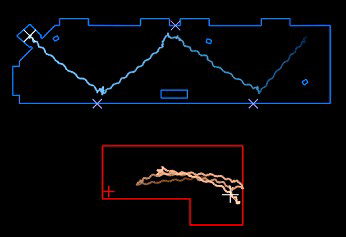
\includegraphics[height=0.8\textheight]{walker-1}\end{figure}\note{This figure shows a small scale example of exploring a larger virtual world in a smaller physical space}}
	\only<2>{\begin{figure}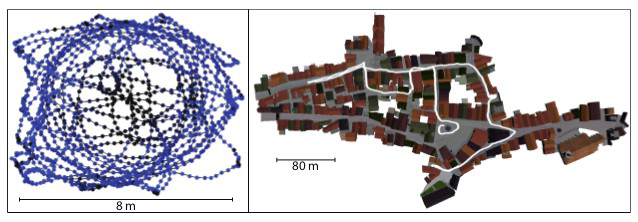
\includegraphics[width=\textwidth]{walker-3}\end{figure}\note{Now, this next figure is a bit more interesting. As you can see, with very limited physical space, people are able to explore a virtual world that is almost two magnitudes bigger.}}
\end{frame}

\begin{frame}{Analyses of human sensitivity to redirected walking}
	\begin{figure}
		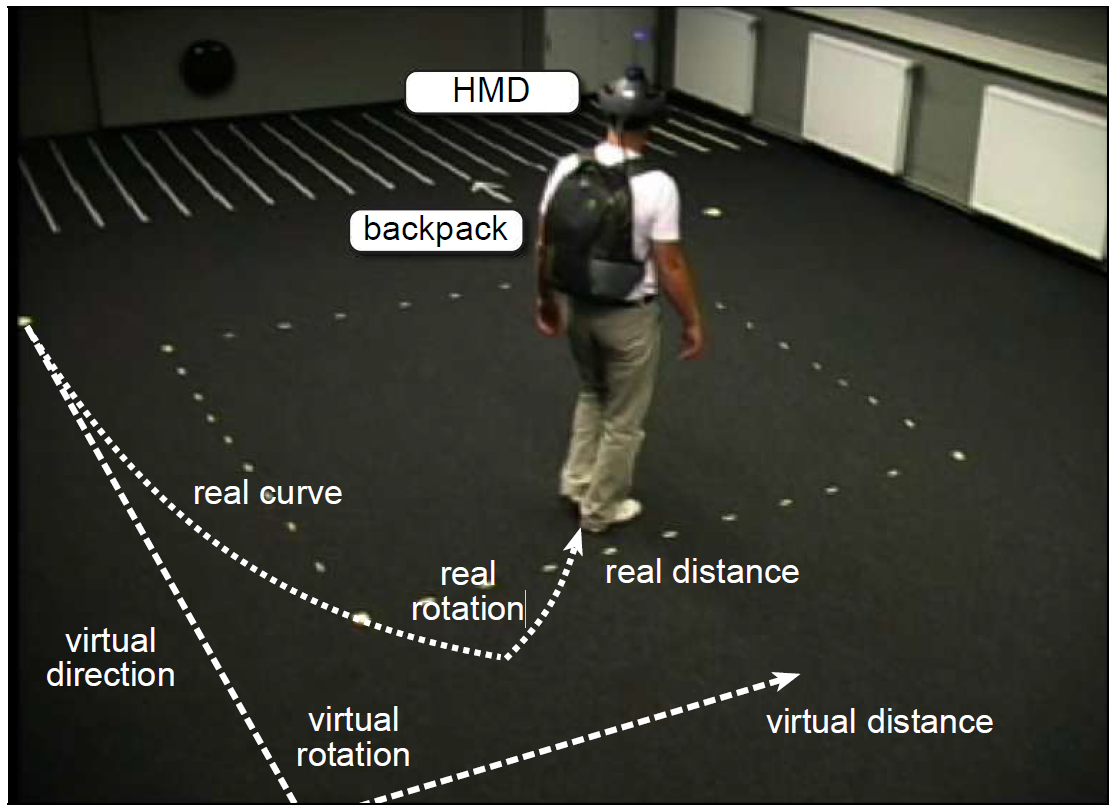
\includegraphics[height=0.8\textheight]{steinicke-1}
	\end{figure}
	\note{So this study laid the groundwork for the work of Walker. As you can see here this is the experimental setup they used.}
\end{frame}


\section{Experiment}
\begin{frame}{Setup}
	\begin{itemize}
		\item Virtual world with a path
		\item Two groups
			\begin{itemize}
				\item Task
				\item Control
			\end{itemize}
		\item Walk through the physical room
		\item Adjust rotational gains
		\item Maintain presence
	\end{itemize}
	\note{
		So, let's get to the experiment that we designed.
		We're keeping as close as possible to the paper we're trying to reproduce of course, while staying within possible.
		
		There's two test group: One that just walks along the path normally, and one that gets some task while doing this, to see if that distracts them from noticing the gains.
		This task can be anything: We were initially thinking about having people count symbols on the walls or having a light that changes color.
		Ultimately, we settled on math problems.
		
		Presence is very important because people need to be really into the world.
		If we can keep the people present in the world, they will not notice it.
		Break the immersiveness.
	}
\end{frame}

\begin{frame}{Challenges}
	\begin{itemize}
		\item Positional tracking
			\begin{itemize}
				\item Bluetooth triangulating
				\item Oculus DK2 positional tracker
			\end{itemize}
		\item Broken Oculus
		\item 2 hours in the lab per week
	\end{itemize}
	\note{
		We've had some problems- ehrm, faced some challenges of course, during implementation.
		
		First off, positional tracking.
		Change world, need to know where they are.
		Bluetooth, Android, XY, slow.
		Luckily, lab DK2, pos tracker.
		Not really.
		Very small res.
		
		Add to that 2 hours blah.
	}
\end{frame}

\begin{frame}{Solutions}
	\only<1>{
		\begin{itemize}
			\item Gamepad \note{
				We gave up on doing real positional tracking, but we tried to keep it as real as possible by only allowing forward motion.
				This means that while people walked using the controller, they did have to rotate their bodies to change direcion.
			}
		\end{itemize}
	}
	\only<2>{
		\begin{columns}
			\column{0.38\linewidth}
				\centering
				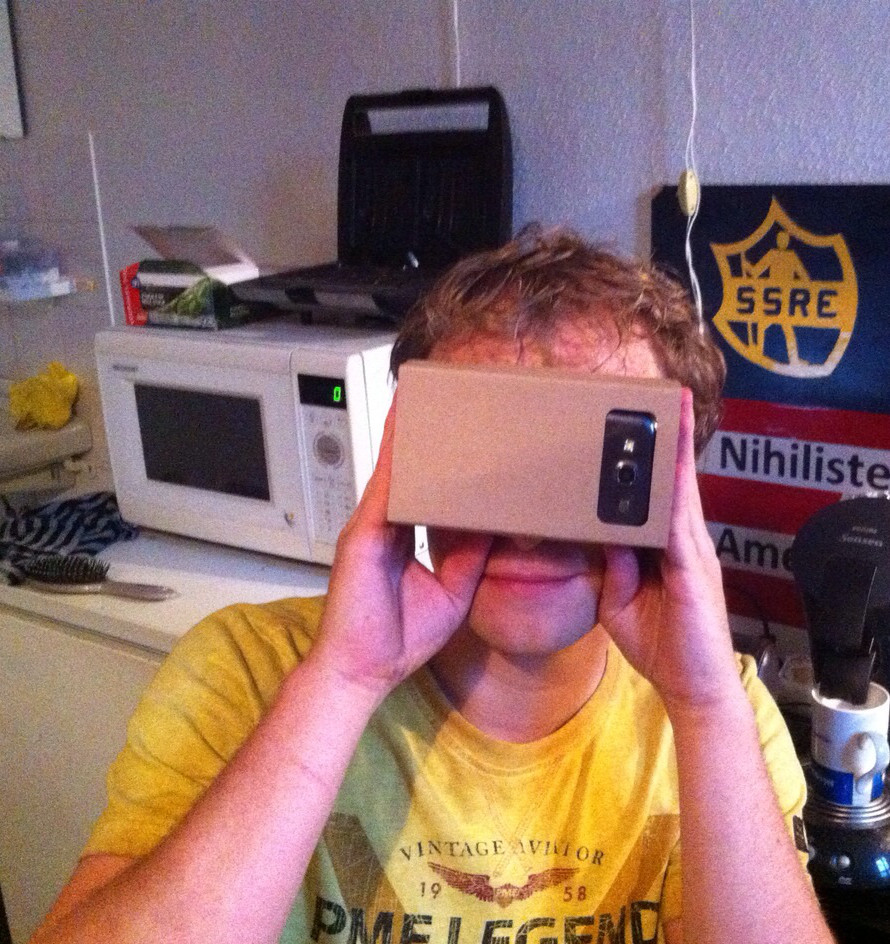
\includegraphics[width=\textwidth]{cardboard}
			\column{0.58\linewidth}
				\begin{itemize}
					\item Gamepad
					\item Google Cardboard (knock-off)
				\end{itemize}
		\end{columns}
	}
\end{frame}

\begin{frame}{Implementation}
	\begin{itemize}
		\item Oculus C++ SDK
		\item Rotational gains
			\begin{itemize}
				\item Change tracking code \note{This happens inside the SDK so not an option\\}
				\item Recalibrate Oculus \note{Not practical because you can't switch easily\\}
				\item Change FPS to influence rotation
				\item Interpret head rotation as extra mouse rotation \note{Weird jump between max and min value, this was noticable for negative gains\\}
			\end{itemize}
		\item Based on \emph{Tinyroom} SDK example
	\end{itemize}
\end{frame}


\begin{frame}{Implementation}
	\begin{figure}
		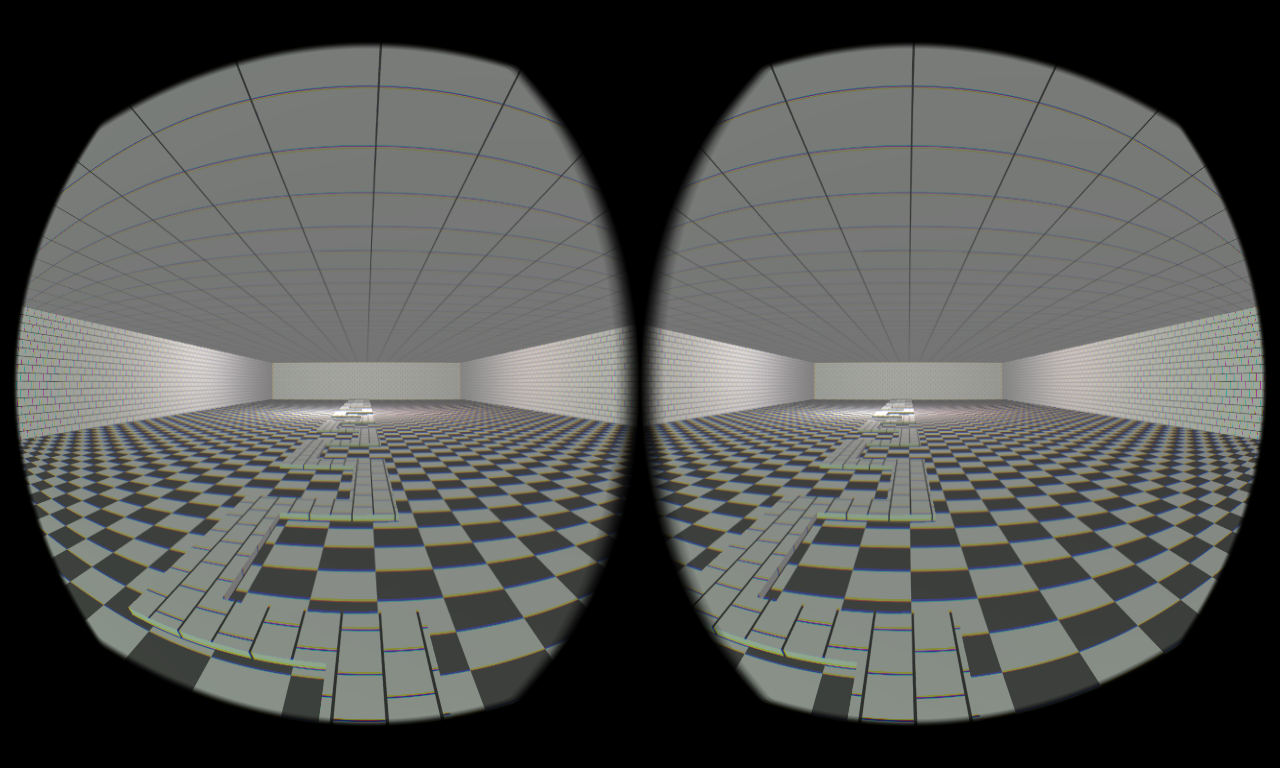
\includegraphics[height=0.8\textheight]{tinyroom}
	\end{figure}
\end{frame}

\begin{frame}{Execution}
	\begin{itemize}
		\item Metaforum
		\item Late at night \note{Because Fontys\\}
		\item Not hard to find subjects \note{Everyone was really excited\\}
		\item But, resetting and calibrating took a long time \note{Because of the jumps\\}
		\item 19 subjects
	\end{itemize}
\end{frame}

\begin{frame}{Execution}
	\begin{figure}
		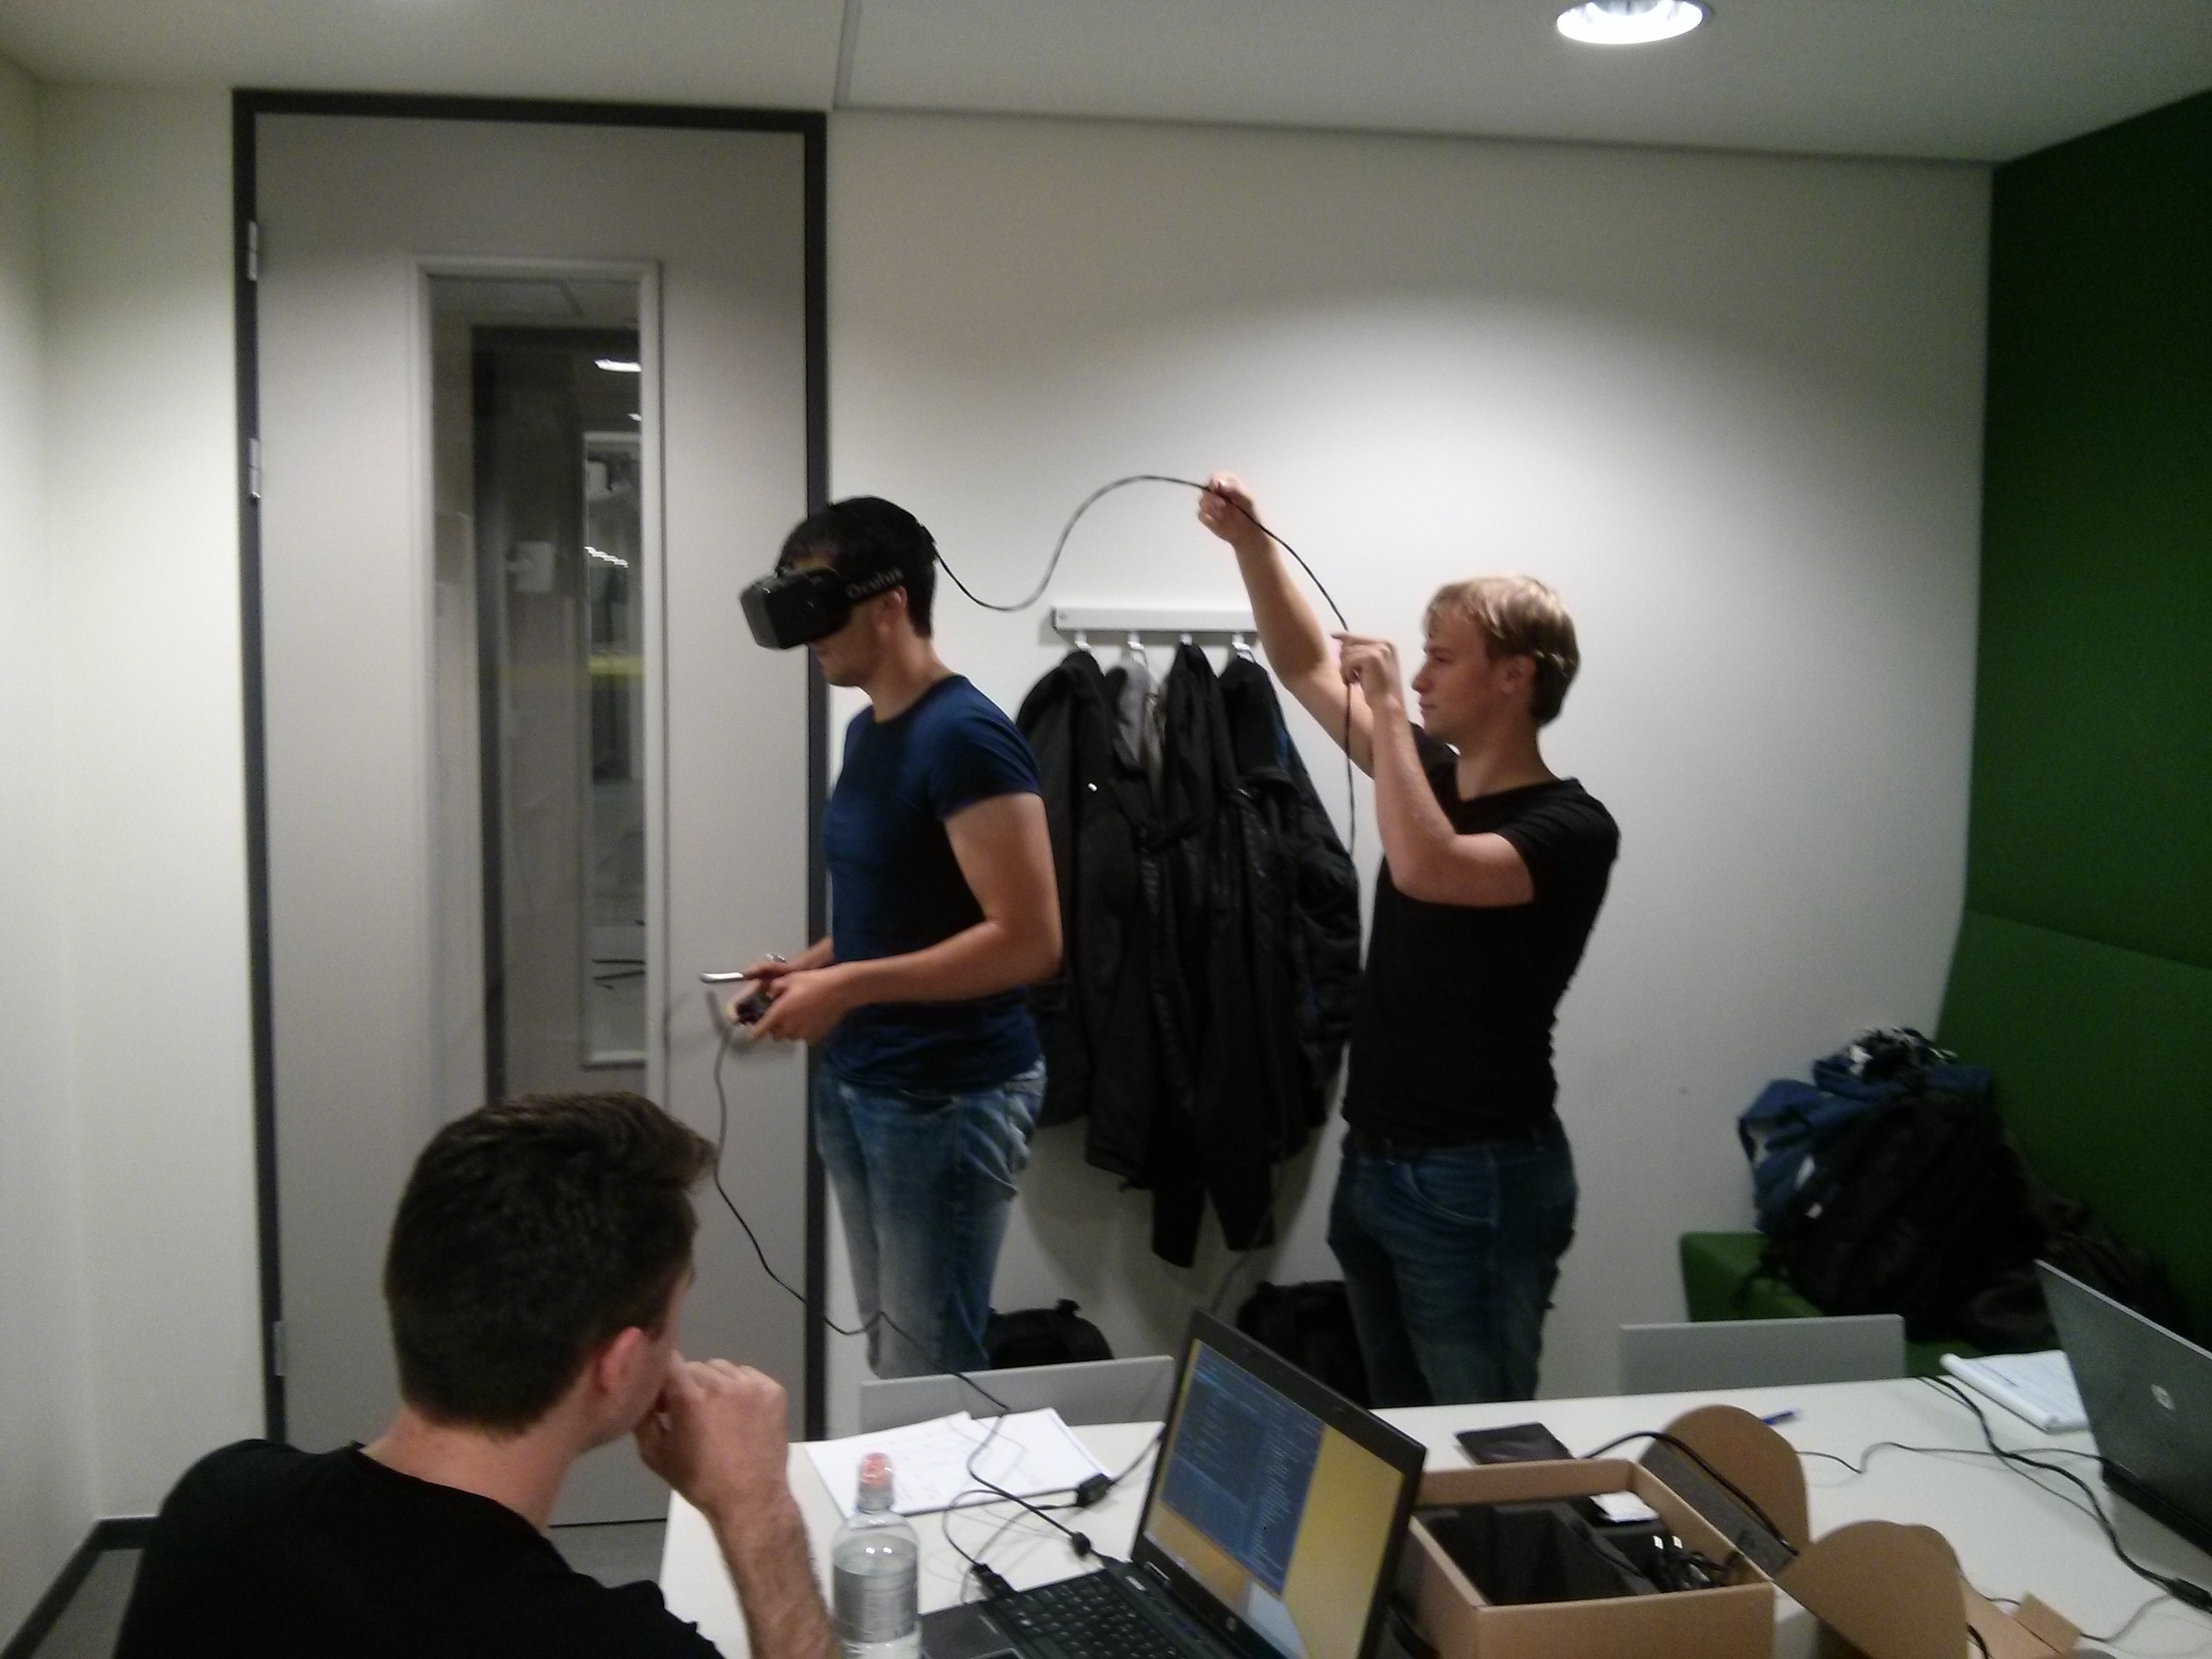
\includegraphics[height=0.8\textheight]{experiment}
	\end{figure}
	\note{Explain how we explained the experiment to the subjects, and what we asked:
		\begin{itemize}
			\item Gain
			\item Gender
			\item Calculation
			\item Notes on condition
		\end{itemize}
	}
\end{frame}


\section{Results}
\subsection{Results}
Now that we have redefined our experiment we discuss the results.
The goal of the experiment is to investigate at what rotational gains the test subjects notice that the virtual world and the real world differ.
Secondly, we are interested in knowing whether this outcome is different when test subjects are engaged in a task (which we have redefined to be simple arithmetic).\\

Now if we look at the results in table 1 we see a couple of columns.
The first column denotes the test subject (or the number of the test).
The second column represents the rotational gain in our implementation, this number is different from the gain as defined by Walker \cite{jwalker}.
Here, 0 means a 1-to-1 mapping from real world to virtual world rotation.
A negative value represents the factor with which virtual world rotation is less than the real world rotation.
Similarly, the positive value represents the factor with which the virtual world rotation is more than the real world rotation.

The third column of table 1 indicates whether or not the test subject did simple arithmetic calculations during the experiment.
Column 4 denotes the test subjects'  response to the following question: ``Did you think your rotation in the virtual world was less, equal or more than your rotation in the real world?"
A ``less" in this column is a correct observation if the gain is negative.
In column 5 the gender of the test subject is shown, we do not conclude anything based on this metric.
In the last column you can see if there are any remarks for the experiment.\\
\\
The first thing that stands out from the results, is that a lot of subjects reported to feeling dizzy or nauseous after the experiment.
Two people felt nauseous, three people felt dizzy and 1 person got a headache doing this experiment.
However, this seems to happen over the entire spectrum of gains tested.
Even though some people seem to be more prone to feeling nauseous from using the Oculus rift then others, having a negative gain (i.e. having to turn further in the real world to achieve a certain rotation in the virtual world) seems to intensify this sensation.
In fact, a test subject opted to stop the experiment due to being very uncomfortable wearing the headset with a negative gain.
This shows us that the human mind might in fact be influenced by the gain.

Especially on the negative gains people felt a little bit sick after (or even during) the experiment.
Even though this is not incorporated in the results we tried the Oculus ourselves with negative gains of up to -0,5 and half of our group got nauseous as well, so when you make the gain too small this has a very negative effect on the body (though we cannot say this for sure since we do not have a lot of tests which confirm this statement).
A possible explanation for this is (including the cases with the positive gain) that people wear the Oculus for the first time in their lives and they have not worn anything like this in their life before.
For a lot of people this technique is really new to them and when you put on the headset a lot of people first have to get used to the Oculus. 
It is not uncommon for some people to have more trouble adjusting to the Oculus than others (especially having different gains).
This could explain the nausea and the dizziness.
People becoming slightly dizzy to the point of feeling nauseous is actually a side effect of the Oculus that has been reported in the media as well.
We also think that the people who wear the Oculus  for the first time are less likely to notice diffrences in the gain, because people who did wear it before can compare the experiment with their previous experience which most likely had no differences in the gains. 

Considering the rotational gain, 3 out of 8 (37.5\%) test subjects correctly noticed a negative gain, 4 out of 8 (50\%) did not notice anything and 1 (12.5\%) even reported a positive gain.
Of the 9 test subjects that experimented with a positive gain, 2 (22.2\%) correctly noticed this, while 6 (66.7\%) did not notice and 1 (11.1\%) even reported a negative gain.
More experiments need to be done to obtain statistically significant results.
From the face of these results, we could say that the negative gain is noticed more often, this is in accordance with our expectations.
We think the people reporting inverse results should be considered outliers.

Another interesting fact is that a lot of people had no notion of what was happening in the virtual world compared to the real world.
In fact it looked the same for a lot of people.
Both the experiment of Walker \cite{jwalker} and ours take place in an empty virtual room with just a path.
It might be interesting to see if the room having additional objects has another effect on the perception of the test subjects
An interesting area for future research is to investigate how the results would differ if the virtual space had more noise, such as buildings or trees around.
Then when a person turns it he or she may notice faster that there is something 'wrong'  with the virtual world.

When we look at the results we see that the group without the tasks 2 out of 9 (22.2\%) noticed the differences in the gain, so 3 out of 9 (30\%)  test subjectives got it correctly.  The group with the task noticed differences in the gain in 6 out of 10 (60\%) times and got it correctly in 3 out of 10 (30\%) times. What is really strange is that the test subjectives of 0.5 and -0.5 noticed completely opposite gains as excepted. The test group without task had 3 out of 9 (30\%) people that felt nauseous or dizzy and the group with task had 4 out of 10 (40\%) people that got nauseous or dizzy. So with a quick glance at the results, we can only mention that there are no significant differences between the test groups, when we compare the correctly noticed differences in the gains and the people that felt dizzy. There is however a big difference between that noticed a difference in the gain, but we do not know for sure if there is a logical explanation or that it is just noise.
\subsection{Comparison to related work}
From our limited test-set, we can not deduce exact negative and positive gains from which the subjects start to notice that the virtual world is different from the real world.
Our result that negative gains are noticed more is in accordance to the study by Walker \cite{jwalker}.
For the possible application of letting people walk around in a large virtual world, but a small physical world, the positive gains are more important and so it is a desirable result that the effects of positive gains are less noticed.


\section{Conclusion}
\begin{frame}{Future work}
	\begin{itemize}
		\item More objects in the virtual world \note{Increase the presence by making the world look more real\\}
		\item Dynamic gains \note{Based on where you are in the virtual world, so different turns, etc\\}
		\item Repeat with people that have used the Oculus \note{Do they know how it should be?\\}
		\item Up and down \note{In our experiment, people didn't have to look up and down. In \\}
	\end{itemize}
\end{frame}

\begin{frame}{Conclusion}
	\begin{itemize}
		\item We can't draw a conclusion
		\item Very different between different subjects
		\item But in our own experience...
	\end{itemize}
\end{frame}

\begin{frame}
\end{frame}


\end{document}
